% !TEX TS-program = pdflatex
% !TEX encoding = UTF-8 Unicode
% !BIB TS-program = biber
% !BIB program = biber

\documentclass[12pt]{article}

%%% PAGE DIMENSIONS
\usepackage[margin=2.54cm]{geometry}
\geometry{a4paper} 
% \usepackage{caption}
% \usepackage{subcaption}
\usepackage{graphicx} % For better graphics
\usepackage{pdfpages} % To insert pdfs into the library
\usepackage{tikz}
\usepackage{wrapfig}
\usepackage{siunitx}

%%% PACKAGES
\usepackage{booktabs} % for much better looking tables
\usepackage{amsmath} % for better maths
\usepackage{paralist} % very flexible & customisable lists (eg. enumerate/itemize, etc.)
\usepackage{verbatim} % adds environment for commenting out blocks of text & for better verbatim
\usepackage{subfig} % make it possible to include more than one captioned figure/table in a single float
\usepackage[framed,numbered]{matlab-prettifier} % enable inserting matlab code.
\usepackage[parfill]{parskip}
%\addtolength{\jot}{1em}
\usepackage{amssymb}
\usepackage{cancel}
\usepackage{color}
\usepackage{listings}

% Create Listing Colours
\usepackage{xcolor}

\definecolor{codegreen}{rgb}{0,0.6,0}
\definecolor{codegray}{rgb}{0.5,0.5,0.5}
\definecolor{codepurple}{rgb}{0.58,0,0.82}
\definecolor{backcolour}{rgb}{0.95,0.95,0.92}

\lstdefinestyle{mystyle}{
    backgroundcolor=\color{backcolour},   
    commentstyle=\color{codegreen},
    keywordstyle=\color{magenta},
    numberstyle=\tiny\color{codegray},
    stringstyle=\color{codepurple},
    basicstyle=\ttfamily\footnotesize,
    breakatwhitespace=false,         
    breaklines=true,                 
    captionpos=b,                    
    keepspaces=true,                 
    numbers=left,                    
    numbersep=5pt,                  
    showspaces=false,                
    showstringspaces=false,
    showtabs=false,                  
    tabsize=2
}
\lstset{style=mystyle}

\usepackage{multicol}
\usepackage{float}

% References
\usepackage[backend=biber,style = numeric]{biblatex}
\bibliography{sources}

%%% HEADERS & FOOTERS
\usepackage{fancyhdr} % This should be set AFTER setting up the page geometry
\setlength{\headheight}{15pt}
\pagestyle{fancy} % options: empty , plain , fancy
\renewcommand{\headrulewidth}{0pt} % customise the layout...
\lhead{University of Auckland}\chead{GOCPI}\rhead{Connor McDowall}
\lfoot{}\cfoot{\thepage}\rfoot{}

%%% SECTION TITLE APPEARANCE
\usepackage{sectsty}

%%% ToC (table of contents) APPEARANCE
\usepackage[nottoc,notlof,notlot]{tocbibind} % Put the bibliography in the ToC
\usepackage[titles,subfigure]{tocloft} % Alter the style of the Table of Contents
\renewcommand{\cftsecfont}{\rmfamily\mdseries\upshape}
\renewcommand{\cftsecpagefont}{\rmfamily\mdseries\upshape} % No bold!

%%% Hyperlinking 
\usepackage{hyperref}
\begin{document}
\begin{titlepage}
	\newcommand{\HRule}{\rule{\linewidth}{0.5mm}} % Defines a new command for horizontal lines, change thickness here
	
	\center
	
	%------------------------------------------------
	%	Headings
	%------------------------------------------------
	
	\textsc{\LARGE }\\[1.5cm] % Main heading such as the name of your university/college
	
	\textsc{\Large University of Auckland\\Department of Engineering Science}\\[0.5cm] % Major heading such as course name
	
	%------------------------------------------------
	%	Title
	%------------------------------------------------
	
	\HRule\\[0.5cm]
	
	{\huge\bfseries Global Optimisation Carbon Pricing Initiative (GOCPI)}\\[0.4cm] % Title of your document
	
	\HRule\\[0.5cm]
	
	%------------------------------------------------
	%	Author(s)
	%------------------------------------------------
	
	{\large\textit{Author: Connor McDowall \\Supervisor: Rosalind Archer}}\\
	
	%------------------------------------------------
	%	Date
	%------------------------------------------------
	
	\vfill\vfill\vfill % Position the date 3/4 down the remaining page
	
	{\large\today} % Date, change the \today to a set date if you want to be precise
	 
	%----------------------------------------------------------------------------------------
	
	\vfill % Push the date up 1/4 of the remaining page
	
\end{titlepage}
\newpage
\section*{Completed Declaration of Contribution Form}
This form is to accompany
\newpage
\section*{Abstract}
\newpage
\section*{Acknowledgements}
\newpage
\tableofcontents
\newpage
\section*{Notion List}
\newpage
\listoffigures
\newpage
\listoftables
\section{Introduction}
\section{Literature Review}
\subsection{An Introduction to Energy}
	Energy powers the world we live in.
Industrial sectors use energy to power machining and production processes. Trade uses oil-based products to fuel shipping and logistics networks. 
The technology sector uses energy to supply power to data centres to facilitate internet services. The manufacturing sector use the chemical properties of oil and natural gas to produce glass, synthetic, and explosive products. 
In summary, energy has a role in every industry. Energy comes in many forms. 
The International Energy Agency (IEA) aggregates energy products into six key fuels: Coal, Gas, Oil, Renewables, Electricity, and Nuclear \cite{W:2}. 
Coal, Gas, and Oil are non-renewable fossil fuels with high energy intensities and carbon emissions. 
Nuclear energy is a non-renewable resource as the uranium used in production is finite. 
Renewables utilise technologies to produce energy from infinitely available wind, solar, geothermal and hydro resources. 
These technologies emit low to no carbon emissions. 
Regardless, energy will power our way of life.

\subsection{Energy, Emissions, and the Economy}
Academics spent decades hypothesizing causal relationships between economic growth, energy consumption, and carbon dioxide ($CO_2$) emissions.
One study explored this hypothesis by applying panel unit root tests, panel co-integration methods, panel causality tests, Fully Modified Ordinary Least Squares (FMOLS), and Dynamic Ordinary Least Squares (DOLS) estimation methods \cite{J:3}.
Another study explored both linear and non-linear causality using Granger Causality and Vector Autoregressive models \cite{J:9}.
Although these modeling techniques are not explored further in this literature review or project, there results show a relationship between economic growth, energy consumption, and carbon dioxide ($CO_2$) emissions.
Subsequently, we must improve our understanding of the three variables and how their relationship informs energy strategy.

\subsubsection{Energy}
Global energy consumption increased annually over the last decade. 
As outlined in BP's Statistical Review of World Energy, world consumption grew from 11705.1 Million Tonnes Oil Equivalent (Mtoe) in 2008 to 13864.9 Mtoe in 2018.
World consumption grew 2.9\% per annum in 2018 and 1.5\% per annum for the period 2007-2017. 
In 2018, 85\% of global energy consumption came from Oil, Natural Gas, and Coal.
Global oil consumption increased by 1.2\%, global coal by 1.4\%, global gas by 5.3\%, global nuclear by 2.4\%, global hydro-electricity by 3.1\%, and global renewables by 14.5\% \cite{TR:3}.
The 14.5\% growth in renewables from 2017 to 2018 highlights how renewables are increasingly competitive as emphasised in the 2020 Deloitte US Renewable Energy Outlook. Flat electricity load growth, declining costs, and the maturation of energy storage
all contribute to decreasing costs and increasing competitiveness. 
Decentralised energy networks with remote renewable micro-grids bolster resilence from increasingly frequent adverse weather events. 
Collaborative efforts lead to newly created efficiencies and the nurturing of new ideas, investment, and leadership. 
The combination of stakeholders' demand for increased resilency in power networks, and collorative efforts to foster innovation in renewables, will continue to drive renewable uptake \cite{TR:4}. \\\\
The fallout from the 2008 financial crisis led to a decrease in global consumption. 
The COVID-19 pandemic is ravaging global oil markets with an approximate 1550 Mtoe (33\% \cite{W:3}) decrease in consumption. 
The fall in demand from COVID-19, and the inability to store more oil, will catalyse significant change. 
Governments are distributing stimulus packages in response to the pandemic. 
Consumption is likely to bounce back after the fallout from COVID-19. 
Stimulus and the disruption to the energy industry may change the way energy is produced and consumed moving forward.

\subsubsection{Emissions}
Greenhouse gas emissions (GHG) are adverse by-products from the production or consumption of fossil fuels. 
Carbon dioxide ($CO_2$) and Nitrous Oxide ($N_2O$) originate from combusting fossil fuels. 
Methane ($CH_4$) is emitted from fossil fuel production processes. 
GHGs act as insulators, slowing the rate energy leaves the earth's atmosphere by absorbing energy. 
Global Warming Potential (GWP) measures how much energy one tonne of gas will absorb relative to one tonne of $CO_2$. 
The GWP for $CO_2$ is 1 and remains in the atmosphere for thousands of years. 
The GWP for $N_2O$ is 265-298 over 100 years. 
Lastly, the GWP for $CH_4$ is 28-36 over 100 years \cite{W:4}. 
Carbon dioxide emissions from the consumption of oil, gas, and coal for combustion increased annually over the last decade. 
This subset of global emissions rose from 30336.7 Mtoe in 2008 to 33890.8 Mtoe in 2018, growing 11.72\% over this period \cite{TR:3}. 

It is hard to argue anthropomorphic contributions to global emissions are not playing a role in climate change. 
The Intergovernment Panel on Climate Change (IPCC) are an intergovernment body of the United Nations (UN). 
The IPCC inform relevant parties on the scientific basis of risk-induced climate change.
The IPCC also convey it's natural, economic, and political implications. 
The IPCC prepared a special report on Global Warming of 1.5 \si{\degree}C, based on an assessment of around 6,000 peer-reviewed publications. 
This report confirms climate change is affecting livelihoods and ecosystems worldwide.
Approximately between 0.8 \si{\degree}C and 1.2 \si{\degree}C of global warming above pre-industrial levels is attributable to human activities. 
It is likely to reach 1.5\si{\degree}C between 2030 and 2052 if the current rate of increase continues. 
The warming from the pre-industrial era to the present will persist for centuries to millennia.
Climate models are predicting increased mean temperatures in land and sea regions, hot extremes, heavy precipitation, drought, and precipitation deficits. 
Biodiversity and ecosystem impacts, such as species loss and extinction, will increase. 
Ocean temperatures, acidity, and oxygen scarcity will increase. 
Global warming will impose risks to health, livelihoods, food security, water supply, human security, and economic growth.
All expected to increase unless severe action is taken \cite{TR:5}. 
Subsequently, emissions will continue to play an important role in our future.

\subsubsection{Economy}
The global economy grew substantially over the last century. 
Worldwide Gross Domestic Product (GDP) per capita (constant 2010 USD) grew from \$3746 in 1960 to \$10891 in 2018 \cite{W:5}. 
Gross Domestic Product increased from \$66.1 trillion (Current USD) in 2010 to \$85.9 trillion in 2018 (Current USD). 
The World Bank segments GDP into four key segments: Agriculture, Industry, Manufacturing, and Services. 
Agriculture corresponds to International Standard Industrial Classification (ISIC) divisions 1-5 which cover forestry, fishing, cultivating crops, and livestock production. 
Industry corresponds to ISIC divisions 15-37 covering mining, manufacturing, construction, electricity, water, and gas.
Manufacturing corresponds to ISIC divisions 10-45 covering businesses which physically or chemically transform materials of components into new products. 
Services corresponds to ISIC divisions 50-99 covering wholesale trade, retail trade, transport, and government, financial, professional, and personal services. 
In 2018, Agriculture, Industry, Manufacturing, and Services made up 3\%, 25\%, 16\%, and 65\% of GDP respectively \cite{W:6}. 
On inspection, energy related products are key inputs to producing segment outputs. 
Traditionally, production is a function of capital and labour. 
Energy should be included in this set with theoretical and time series analysis supporting this claim. 
Empirical and theoretical evidence suggests energy availability, coupled with energy use and output, plays a key role in enabling growth \cite{J:4}.
Unfortunately, the COVID-19 pandemic drew to a close this period of unprecedented growth as the economy is forecast to plunge into a deep recession. \\\\
It is clear action must be taken to reduce anthropomorphic emissions while meeting the needs the economy after reviewing energy, emissions, and the economy.

\subsection{Current Political Action}
\subsubsection{Paris Agreement}

Over the last few decades, there has been debate on anthropomorphic emissions causing climate change. 
During this period, the UN began the United Nation's Climate Change Regime to ratify global agreements to combat climate change. 
There have been three major phases to this regime. 
The first phase was negotiating, adopting, and ratifying the United Nations Framework Convention on Climate Change from 1990 to 1995.
The second phase was the adoption of the Kyoto Protocol on the 11th of December 1997. 
Unfortunately, the protocol took until the 16th of February 2005 to be ratified due to a complex ratification process. 
The Kyoto Protocol operationalized the United Nation's Framework Convention on Climate Change. 
Industrialised countries were committed to reduce and limit GHG emissions in accordance with targets agreed on an individual basis. 
The protocol only bound developed countries as they were deemed mostly responsible for the state of emissions. 
The protocol was split into two commitment periods. 
The first set binding emission targets for 36 industrialised countries, and the European Union, to reduce 5\% of emissions compared to 1990 levels.
The second commitment was set by the adoption of the Doha Amendment on the 8th of December 2012. 
This commitment was set to start 2013, end in 2020, and reduce emissions by 18\% from 1990 levels. 
Unfortunately, the second commitment period was not ratified. 
The protocol established three flexible market mechanisms; International Emissions Trading, Clean Development Mechanisms, and Joint Implementation. 
The protocol held parties accountable by establishing rigorous monitoring, review, verification, and compliance systems \cite{W:7}.

This protocol was a step in the right direction but there were some inherent issues. 
A complex ratification process limited uptake. 
Participating countries had disproportionate obligations to reduce emissions. 
The commitment periods did not have a long term outlook, contained different subsets of participants, and were not global in nature.

There was another long term co-operative action promoted under the UNFCCC, launched in the Bali Action Plan. 
Both the second commitment and the co-operative action were to conclude at the 2009 Copenhagen Conference. 
However, this conference ended in disappointment as there wasn't enough time before the conference to resolve the issues in the regime.

At the conference, the Copenhagen Accord, political in nature, was agreed upon on the final night by a group of states including most major economies. 
This accord established a bottom up architecture where both targets and actions were set individually then reported internationally. 
In 2010, the Cancun Agreements incorporated the Copenhagen Accord into the UNFCCC regime. However, all progress to date did not look pass 2020. 

This issue was resolved at the 2011 Durban Conference when the Durban Platform for Enhanced Action launched the negotiations which lead to the Paris Agreement. 
Negotiations continued for years, addressing how to develop an instrument suitable for all parties, and requested the submission of nationally determined contributions (NDCs)\cite{J:5}.

The 2015 United Nations' Climate Change Conference was held in Paris. 
After some exceptional negotiating from French Foreign Minister Laurant Fabius, the Paris Agreement was adopted on the 12th of December 2015, and ratified on the 4th of November 2016.

The Paris Agreement's main objective is to strengthen the global response to climate change by keeping the temperature rise this century below 2\si{\degree} above pre-industrial levels. 
The agreement also pursues efforts to limit the increase to 1.5\si{\degree}. 
The agreement addresses the following across 29 articles: long term temperature goals, global peaking targets, mitigation efforts through nationally determined contributions (NDCs), sink and reservoir use, market/non-market approaches, adaptations, loss/damage mitigations from the 
adverse effects of climate change, financial support, technology support, capacity-building support, education, reporting systems, and global stocktake procedures \cite{W:8}, \cite{TR:6}. 
Article six of the Paris Agreement outlines mitigations and NDCs which include the following carbon pricing initiatives: Emissions Trading Schemes and Carbon Taxes.

\subsubsection{Carbon Pricing Initiatives}
Emissions Trading Systems (ETS) facilitate emission reductions where cheapest.
Polluters who find it easier to reduce emissions can sell emission allowances to polluters who struggle to lower emissions. 
There are two types of ETS. Firstly, Cap and Trade. Secondly, Baseline and Credit Systems. 
Cap and Trade sets an upper limit on emissions with emission credits either grandfathered or auctioned. 
Most emission credits under this system are grandfathered with proceeds captured by existing polluters. 
Most cap and trade systems are localised regionally or nationally. 
However, the European Union (EU) implemented the EU ETS to trade across the EU.
Baseline and credit systems don't have a fixed level of emissions. 
Polluters can reduce emissions to earn credits to sell to other polluters who need to meet regulations \cite{J:6}.

Carbon Taxes are either implicit or explicit. An implicit tax is incorporated into the price of a GHG intensive product e.g. retail fuels. 
An explicit tax is a price per quantity of emissions produced e.g. \$10 per tonne of $CO_2$ equivalent.

Carbon pricing initiatives are increasingly recognized as instrumental to cost-effectively deliver the transition to low-carbon societies. 
The Organisation for Economic Co-operation and Development (OECD), International Monetary Fund (IMF) and the IPCC all recognise the need to strengthen these initiatives.

57 carbon pricing initiatives are either currently implemented, or scheduled for implementation, as at April 1st 2019. 
28 ETFs are spread across national and subnational jurisdictions with 29 carbon taxes primarily implemented at a national level. 
These pricing initiatives only cover approximately 20\% of Greenhouse Gas Emissions (11 Gt$CO_2$e). 
There is variation in carbon prices from less than US\$1/t$CO_2$e to US\$127/t$CO_2$e. 
Unfortunately most carbon tax price increases are linked to inflation only. 
Governments raised more than US\$44 billion in carbon pricing revenue during 2018.
There are determined price trajectories that can deliver on the Paris Agreement which increase each decade on a non-discounted basis.
IPCC trajectories show the marginal cost of reducing GHG emissions.
Other sources provide carbon price ranges which consider ambitious climate policy.
When setting carbon prices, local, ethical and distribution factors must be considered.

Internal carbon pricing is increasing in popularity within the private sector. 
1300 companies, including 100 Fortune 500 companies, disclosed the current use or intent to use internal carbon pricing. 
Traditionally, internal carbon pricing drove investment planning for mandatory carbon policies. 
Internal carbon pricing is transitioning towards informing long-term climate investment and risk strategies.
Financial policy frameworks are reassessed to use carbon pricing to support sustainable growth. 
Internal carbon pricing is informing the construction of market indexes e.g. S\&P Carbon Price Adjusted Index to inform market climate risk.
Internal carbon pricing will continue to catalyse both the investment in sustainable technology and the divestment in fossil fuels.
Although new carbon pricing initiatives are emerging with an increased emphasis on global collaboration, it is clear the global community is far from reaching the objectives set by the Paris Agreement. 
Only 5\% of carbon pricing initiatives are currently priced to meet the Paris Agreement's temperature goals \cite{TR:7}.

\subsection{Opportunities and Challenges}
\subsubsection{Market-Based Approaches}
Both carbon pricing initiatives are market-based and can be less obtrusive for industry than regulatory controls. 
The prevalence of emissions across global industries sees a market-based approach more equitable, evenly distributed across industries, and quicker to implement.

Arguably, a carbon tax is the most straightforward approach. 
A carbon tax could be imposed on all emitting inputs and outputs of production.
The marginal cost of carbon would be covered by a tax rate. 
Tax credits from sequestration or other initiatives could be used to invest directly into alternative technologies. 
Tax rates could be adjusted to illicit the desired market response. 
A carbon tax would align with existing systems used to facilitate inland revenue functions in the desired jurisdiction.

The effectiveness of cap and trade systems is undermined by grandfathering credits, using offsets in lieu of meaningful emission reduction targets, and the challenges of setting baselines.
If credits are grandfathered, there are no tax revenues to invest in alternative energy or technology.
In a cap and trade system, there is uncertainty around the price of those reductions, and the subsequent effect these credits have on lowering emissions.
Cap and trade initiatives provide benefit certainty as you can ascertain the environmental benefits from an imposed ceiling on emissions. 
However, there is no cost certainty which is provided through a carbon tax.

\subsubsection{Benefits and Costs to a Carbon Tax}
A carbon tax is simpler as is set at a cost per t$CO_2$e produced. 
In contracts, a cap and trade is more complex due to negotiating baselines, grandfathering/auctioning processes, monitoring systems, international trading guidelines, and cost uncertainty prevention.
A carbon tax more easily generates revenue to invest in reducing greenhouse gas emissions and supporting businesses adopting more sustainable processes. 
A cap and trade system generates revenues using credit auctioning but is less effective than a carbon tax if grandfathering credits exists.
A carbon tax ensures cost certainty as the exact cost of emissions is quantified. 
In addition, there is a clear message to polluters with a carbon tax. 
Under a cap and trade system, there is more uncertainty around the impact polluters have as they can merely purchase more credits to increase emissions.
In light of these positives, there are also negatives to a carbon tax. 
There is significant political opposition in proposing a new form of tax. 
The benefits of a carbon tax will need to be clearly communicated to all stakeholders. 
The benefits of a carbon tax are uncertain in how they enact reductions in emissions. 
Tax exemptions may reduce the effectiveness of the carbon tax if granted inequitably. 
For example, if a super major was given a significant tax exemption on the basis of an existing political relationship.
A carbon tax is also difficult to co-ordinate with other participants \cite{J:6}. 
In addition to these disadvantages, there are misconceptions leading to the opposition of carbon taxes. 
These misconceptions include, but are not limited to, the following: Taxes reducing welfare, and increasing unemployment, from lower levels of consumption and production. 
Taxes perceived to put incumbents' business models at risk. Subsequently, these incumbents lobby heavily prevent change.
Taxes increasing the prices of goods and services consumers consume, creating opposing public opinions \cite{A:3}.

Addressing the disadvantages and misconceptions of a carbon tax would help implement carbon taxes across geographies to reduce greenhouse gas emissions.

\subsubsection{Decarbonization, Investment, and Technology}

The revenue generated from carbon taxes would need to be reinvested to benefit regional, national, and global communities. 
One opportunity is investing in sustainable technologies. 
Fortunately, this type of investment is increasing. 
Between 2010 and 2019, renewable technology drew \$2.6 trillion in investment. 
In 2019, \$282 billion of renewable capacity was financed worldwide. 
Wind technologies (onshore and offshore) and solar were financed \$138 billion and \$131 billion respectively. 
This financing success was attributable to falling costs and maturing technologies. 
Renewable technologies are now profitable. 
Costs associated with solar and wind technologies have fallen 85\% and 49\% respectively in the last 10 years \cite{W:10}.
In Australia, New Zealand, Canada, Europe, Japan, and the United States, sustainable investments reached assets of \$30.7 trillion in early 2018, one-third of total investment.
By 2025, renewables will be competitive with natural gas. New technology is emerging in the Oil and Gas Industry to decarbonise the industry. 
These technologies include but are not limited to: renewable power sources, electrification, vapor recovery units, carbon capture, carbon storage, and green hydrogen \cite{A:2}. 
Carbon tax revenues could be used in the following ways: investment into sustainable technologies, replacing existing infrastructure to support sustainable technology growth, reinvestment into participating businesses, or addressing the adverse affects of climate change.
It is important to communicate the benefit of sustainable investment to all relevant stakeholders.

\subsection{Energy Modeling}
It is important to understand how energy demand and supply is modeled before discussing emission levels, carbon taxes, and reinvestment opportunities.
Unsurprisingly, energy modeling is complex.

\subsubsection{Global and Domestic Energy Scenarios}
Different scenarios define modeling processes. 
The World Energy Council devised three energy transition scenarios describing plausible pathways for the global energy transition to follow. 
The scenarios look forward to 2060. There is an inflection point in 2040 to assess the success of the strategies underpinning the scenarios.
The council leveraged expert member communities and annual surveys to devise these strategies.
The three global scenarios tell different narratives relating to the progression of global primary energy demand, electrification,mobility improvements, energy efficiency, infrastructure innovation, investment, new technologies, political action, and Paris Agreement alignment.
There are three global scenarios: Modern Jazz, Unfinished Symphony, and Hard Rock. 
Modern Jazz is a market driven scenario. 
Unfinished Symphony is a highly collaborative, policy driven scenario. 
Hard Rock is a minimally collaborative, internal policy driven scenario \cite{TR:8}.

Countries use the global scenarios to inform their regional and national scenarios. 
New Zealand has followed this methodology through devising the Tui and Kea scenarios. 
Tui follows the narrative of a global community effort. 
New Zealand does not generally have a common view on what is important.
Subsequently, the country adopts a wait and see approach with some protection provided to local businesses.
New Zealand will focus firstly on economic prosperity and individually wellbeing by leveraging off comparative advantages.
This is purely a commercial response. 
Kea forecasts the New Zealand economy cannot remain internationally competitive under current emission intensity trends.
The country will take leadership in lowering emissions, choosing to undergo an early and aggressive economic transformation.
New Zealand will act before the global economy at the expense of its own.

Both scenarios are underpinned by 19 critical uncertainties. 
These vary from external sources such as global stability, international fuel markets, urban sustainability, energy affordability, and the allocation of natural resources. 
Both scenarios consider different service demands e.g. Number of km travelled, population, GDP (\$), forecast carbon prices (\$/t$CO_2$e), carbon emissions (Mt/p.a), required investment (\$), and commodity prices \cite{TR:1}, \cite{TR:2}.
These scenarios were feed into The Integrated MARKEL-EFORM System (TIMES) model to forecast their impact.

\subsubsection{The Integrated MARKEL-EFORM System (TIMES) Model}
The Integrated MARKEL-EFORM System (TIMES) model generator was developed as a component of the International Energy Authority's (IEA) Energy Technology Systems Analysis Program (ETSAP). 
The IEA-ETSAP uses long term energy scenarios to conduct comprehensive environment and energy analyses \cite{J:7}.
Energy is modeled through combining complementary technical engineering and economic approaches. 
TIMES uses a technology rich bottom up architecture, using linear programming to produce least cost energy systems for medium to long term time horizons \cite{J:8}.
The TIMES model encompasses each step in the value chain to produce and supply energy to meet the demand for energy services by consumers.
These include: primary resources, transformation processes, transportation methods and conversion processes. 
The supply side considers production methods and net exports. 
Energy is carried through to residential, commercial, agricultural, transport, and industrial sectors. 
The relationships between producers and consumers underpin the TIMES model. 
The nature of these relationships are mathematical, economic, and technological. 
TIMES considers technologies, commodities, flows, and scenarios constrained by policy decisions.
Services demanded by consumers are the main inputs for the model.
The model will make investment, supply, trade, and operating decisions when considering the inputs, constraints, and scenarios in the model. 
Consumer and producer surpluses are maximized from a mathematical perspective.
The main outputs are energy system configurations at the lowest cost that meet end users' service demands. 
These include energy prices, flows, emission quantities, capacities, and costs \cite{J:8}, \cite{W:12}.

The TIMES model is useful for using energy scenarios to devise strategies for implementing carbon taxes.

\subsubsection{General Algebraic Modeling System (GAMS)}
GAMS is a high-level modeling system for optimization and mathematical programming.
The system is suitable for large scale, complex modeling applications. 
The system gives you access to a diverse portfolio of solvers to solve linear, non-linear, and mixed integer optimization problems.
GAMS is the ideal tool for modeling energy and carbon tax scenarios using TIMES Models \cite{W:11}.

\subsubsection{Open Source Energy Modeling System (OseMOSYS)}
The OseMOSYS project is an open source project to improve the accessibility of modeling energy systems.
The modeling methodology is scalable from city to continental granularities. The approach is designed to require no upfront investment,
little time commitment and provides a fast learning curve. This methodology is suitable for developer, modelers, academics and policy makers.
The model structure includes pre-defined sets, parameters, objective function and constraints relating to energy systems. 
Python, GNU MathProg and GAMS versions are available
for download in remote repositories on Github \cite{W:13}.
\newpage

\section{Project Scope and Research Objectives}
The literature led to some interesting outcomes. 
Carbon taxes are an effective way to help meet the goals set by the Paris Agreement, reduce global emissions, and reinvest in both sustainable and decarbonizing technologies.
However, there are significant obstacles stopping the implementation of carbon taxes. 
These obstacles include political opposition, effectiveness in reducing emissions, co-ordination with other local, regional, national and international carbon tax efforts, and the distribution of tax exemptions.
Currently, the distribution and implementation of carbon pricing initiatives is inequitable as major polluters aren't enforcing these initiatives e.g the majority of the US and India.
Producers who operate globally may pivot to produce and sell GHG intensive products elsewhere in the world if taxes are not correctly set and spread amongst geographies.
In this context, geographies are defined as geographical areas where energy consumption and emission production occurs. 
Earth is the entire set of geographies.
This set can be partitioned into continental, national, provincial, or regional geographies (subsets).


Any carbon pricing initiative must consider the specific combination of energy factors for the associated geography.
The aggregate outcome from all geographies should meet the objectives set by the Paris Agreement.
The revenues generated should be distributed back to participants with commercial benefits communicated through key financial metrics relevant to that geography or business.

The overall research objective is: 
\begin{center}
\textbf{Develop a Global Carbon Pricing Optimisation Model}.
\end{center}

The model will be developed by the following process:

\begin{enumerate}
	\item Understand the existing approach to forecasting services demand and develop a standardised forecasting process which aligns with emission targets
	\item Partition the global set of geographies into subsets with varying levels of granularity e.g. a continental subset with seven geographies (continents), a national subset with 195 geographies (sovereign states according to the United Nations) etc
	\item Forecast services demand for each geography in each subset
	\item Adapt an existing TIMES/OseMOSYS model to input standardised energy system parameters 
	\item Run simulations using the adapted model to form distributions on model outputs. These distributions are to inform the negotiation of carbon pricing initiatives
	\item Develop and model investment strategies from subsequent key outputs including carbon prices
	\item Develop a model interface (UI and UX) to communicate optimal global carbon prices, performance metrics, and the carbon tax benefits to support co-ordinated efforts to negotiate and implement carbon pricing initiatives 
\end{enumerate}

In conclusion, this project will attempt to address issues surrounding climate change. 
GOCPI will enable any user to design and model their own energy system to inform investment and policy decisions.
The intention is to empower users to influence energy investment and policy decisions made by public and private parties.

\section{Methodology and Implementation}
\subsection{Project organisation}
GOCPI adopted Data Science best practice, as described by Wilson et al \cite{J:10}. Although these practices are
mostly reserved for data science projects, their principles are suitable for product development and version control. All data and
results are saved regularly and reproducible. The retention of data in all forms received high levels of attention. Project files were synched
continuously to Google Drive \cite{Google_Drive}. Git \cite{Git} was used to manage version control for GOCPI's source code, data, documentation and results.
Git stores a complete history of versions using Git hashes. These hashes are strings unique to each state of the
publicly available GOCPI repository\footnote[1]{https://github.com/CMCD1996/GOCPI}. Git hashes enable the discretisation of GOCPI's development over time,
enabling the accessibility and recollection of all previous states given a unique git hash. This functionality
enables reproducibility, error correction and the ability to revert to previous models.

\subsubsection{Version Control}\label{Version Control}
Git, hosted by GitHub, provides a comprehensive set of version control technologies. These technologies provide a range of benefits.
Firstly, Git is excellent at providing and supporting collaborative functionalities. The master version of a project is accessible for all
who have access to the repository. Each contributor can create custom copies of branches through pull requests on the master branch. Contributors
can commit changes to custom branches and push these changes to the master branch through push requests. The product manager can review these push requests,
approving suitable requests to integrate changes to the master branch. Collaborative efforts were possible with
commit messages describing the contributions from each contributor. This project had one contributor. Git ensures the histories of code, work and authors are stored.
The descriptive nature of the commit log ensures an accurate journal is kept.

\subsubsection{Folder Structure}
GOCPI maintained the file folder structure recommended in Wilson et al \cite{J:10}. Project organisation was paramount as the modelling of energy systems involves
integrating a range of optimisation models, data files and documents. Wilson et al's recommendations were appropriate as data science projects require similar 
organisational rigor. Subsequently, file management and structure was most efficient and comprehensive. \textbf{GOCPI} is the root directory of this project and contains several
sub directories: bin, data, doc, src and results.  The \textbf{bin} subdirectory contains external scripts and compiled
programmes related to the GOCPI project. The \textbf{data} subdirectory contains all raw data associated with the project. 
This data includes energy statistics, energy balance datasets, partitioned geographies, standardised optimisation models and TIMES modelling frameworks.
The \textbf{doc} subdirectory stores GOCPI's user guides, academic resources, research reports and project deliverables.
The \textbf{results} subdirectory contains the output from optimisation simulations and processed data to display on dashboards and websites to inform investment and policy decisions.
The \textbf{src} subdirectory stores the source code for preparing raw data, partitioning sets of geographies with varying granularities and the
GOCPI python package available to download using PyPI\footnote[2]{https://pypi.org/} and install using pip\footnote[3]{https://pypi.org/project/pip/}.
All files were continuously backed up using Google Drive.

\subsubsection{Python}\label{python}
Python 3.7 was the primary coding language for the GOCPI project. 
GOCPI's objective is to enable any user to design and model their own energy system to inform investment and policy decisions.
The intention is to empower users to discuss energy investment and policy decisions made by public and private parties.
Additionally, GOCPI intends to reduce misinformation regarding energy policies and help assess the feasibility of meeting the International Energy Agency's Sustainable Development Scenario \cite{IEA_WEM}.
Python is omnipresent, widespread in software development. 
Python's language design makes the language highly productive and simple to use. 
Python can hand off computationally straining tasks to C/C++ and has first-class integration capabilities with these two languages.
The language also has a very active and supportive community \cite{Python_Features}.
In addition, Python is the most popular coding language on the planet defined by the PYPL PopularitY of Programming Language Index. As at August 2020, Python had 31.59\% of all language tutorial search instances on Google \cite{PYPL_Pop}.
Python has many useful packages for creating the GOCPI package such as NumPy, Scikit-learn, os, csv and Pandas. 
Programming is quick due to Python's dynamic nature.
The language is also open-source with no cost.
Subsequently, the GOCPI model should be accessible for many users to use and extend.

\subsubsection{Package Management}
The Anaconda package management platform for Python \cite{Anaconda} was the chosen coding environment.
Anaconda is a well defined, free platform with known versions of python packages such as matplotlib, numpy and pip.
The use of this environment ensures both reproducibility and consistency across infrastructure.
These factors enable collaborative efforts. 
Although this project required no collaboration, the use of Anaconda will inform future developers on how to manage collaborative processes, especially for packages
which are less well-maintained. Anaconda allows you to create custom environments which was necessary for creating scalable linear optimization problems to express energy systems.
Pip is Python's default package manager and included within the Anaconda package. 
Pip was used to install and update packages for python not available on Anaconda such as twine and the custom GOCPI package developed for this project.

\subsubsection{Excel}
It is important users are comfortable with using the GOCPI model. 
Energy modelling can be quite complex. The modelling process must be transparent to inform users how to build their own models.
Excel is ubiquitous across academic and professional communities.
Excel's omnipotence makes the software well-suited for describing the components of the GNU Mathprog energy system model.
The \textbf{GOCPI OseMOSYS Structure.xlsx} file describes the sets, paramaters, constraints and objective function of a scalable energy system model.
The User may toggle statements sets, parameters and constraints to change the complexity of the model. 
The model is imported to a text file using the \textbf{CreateModelFile} module in the \textbf{GOCPI} package.
However, data related to these energy systems is stored using Python dictionaries, lists and NumPy arrays.
Excel is best for two dimensional variables or data stored in Codd-Boyce relational databases \cite{CBNF}.
Many of the parameters in energy systems modelling contain three or more dimensions. 
Therefore, Excel is not suitable to store these parameters.
Python dictionaries, lists and NumPy arrays are preferred alternatives.

\subsubsection{IBM ILOG CPLEX Optimization}
The OseMOSYS methodology (see \ref{OseMOSYS}) translates energy systems into linear programming problems. A solver is required to optimise these user-defined energy systems.
The IBM ILOG Optimization Studio \cite{IBM_ILOG}, more commonly known as CPLEX, was chosen to be this solver.
CPLEX solves very large linear programming problems using the Barrier Interior-point method \cite{IPM} or primal/dual variants of the Simplex Method \cite{Simplex}.
GOCPI's user-defined energy systems can be scaled up to model very large systems, creating large linear programming problems.

The IBM ILOG CPLEX Optimization Studio has an interface with the Python language based on a C programming interface.
Subsequently, Python APIs are available to run the CPLEX solver when installed either locally or on a cloud service.
The python packages are \textbf{cplex} and \textbf{docplex}. The cplex package contains classes for accessing CPLEX for the Python programming language. 
The Cplex class is the most important class in this package as provides methods for creating, modifying, querying, or solving optimisation problems.
Docplex also enables the formulation of new linear programmes where one creates the model, defines the decision variables, sets the constraints and expresses the objective function.
The user uses docplex to solve the linear programme on a local solver. 
Alternatively, the model can be solved on a private cloud using Decision Optimisation on Cloud service through the provision of a service url and personal API key.
The CPLEX Python APIs are most attractive as provides the user with a powerful commercial solver in an accessible format.

There is a caveat to the use of the CPLEX solver. The IBM ILOG CPLEX Optimization Studio is commercial by nature and requires a license to use.
Fortunately IBM have the IBM Academic Initiative \cite{IBM_AI}, granting students access to commercial software for free.
This commercial nature creates accessibility issues for users who are not enrolled at an academic institution or can afford to pay for the software.
Accessibility issues caused by the need for commercial solvers must be addressed to enable the distribution of the GOCPI product.

\subsubsection{IBM Watson Machine Learning Service}
The IBM CPLEX Optimisation Cplex python API is suitable for smaller models that can be solved locally.
As the model increases in complexity, the docplex Python API did enable the ability to solve larger linear programmes.
Unfortunately, IBM have phased out the docplex Python API by incorporating Decision Optimisation on Cloud services into the IBM Watson Machine learning cloud services \cite{IBM_WML}.
This change occurred very recently
This service uses IBM Cloud to access assets through credentials, create model deployments in IBM's servers and execute jobs to solve models.
The model deployments must be Python-based models with jobs specifying a payloads containing input data.

\subsubsection{PyPI}
PyPI\footnote{https://pypi.org/} is the Python Package Index, a repository of software for the python programming language.
This repository helps you find and install software developed by the Python community who have decided to share their work.
The GOCPI package is distributed from this platform to enable as many as possible the ability to model their own energy systems to inform and question energy policy and investment.
Enter command: \textbf{pip install GOCPI} in the terminal to install the package using pip package management software.

\subsubsection{Code Style}
The GOCPI project is developed as the GOCPI package where all development code is organised.
The PEP8 style for Python Code is the formatting style for development code \cite{PEP8}. 
All code is formatted with \textbf{yapf}, a formatter maintained by Google to format created Python files.
Standardised formatting is important as makes the code easy to read, helps optimise the code and promotes consistency.
Docstrings and commenting were most important in documentation. A docstring is a Python inline comment. 
Each class and function has an unique docstring, a one sentence description of the function, inputs with data types and types of outputs.
The Google style docstring was most appropriate because of it's readability, ease to write and consistency with the Google Style Guide.
Additionally, automated documentation generators (\textbf{pdoc3, Sphinx} etc.) can parse this format to create documentation.
This self-consistent code style facilitated best practise maintenance and enables reproducibility.


\subsubsection{Infrastructure}
GOCPI creates scalable energy system optimisation models which change in complexity depending on there size.
Computations either took place locally on a 128 GB, four core Apple MacBook Pro or remotely using a cloud service. 

\subsection{Documentation}
The GOCPI project is well documented to keep an accurate record of key design decisions.
The commit history described in \ref{Version Control} was the most important form of document.
Other explicit documentation methods were applied to supplement this commit history. 
These methods, in addition to in-code documentation, include project updates and meeting minutes
nested with a project logbook.

\subsubsection{Project updates}
Project updates were recorded as itemized lists.
Each item is a brief description of the work completed during that day, week or month.
Items include, but are not limited to, completing GOCPI submodules, researching energy system statistics, building websites or writing sections of this research report.
These updates were pivotal to exploring new options, monitoring progress and making decisions to drive forward development. 
For example, the decision to adopt the OseMOSYS methodology in favour of the TIMES modelling methodology.
Project updates were transcribed to the project logbook held in this project's research compendium.

\subsubsection{Meeting minutes}
Project meetings took place for half an hour once a week. 
These meetings included discussions on energy markets, modelling methodologies, project progress and key design decisions.
The minutes from these meetings accompanied project updates in the project logbook nested within the research compendium.

\subsection{Geographical Partitioning}
The first stage of the GOCPI project was to come up with an exhaustive list of geographies. 
The user has the choice to either model the energy systems of these geographies individually or model a network of geographies connected by trade relationships.
Geographies are grouped into three distinct sets. There is a continental set with six continents: Africa, North America, South America, Oceania, Asia and Africa.
Antarctica was excluded from this set.
The country set includes 194 United Nations member states. The elements in the city set number approximately 13800 unique cities from the 194 member states.
The \textbf{GOCPI Geographies.gyp} script processes these unique sets to create a csv file detailing an aggregate geography set.
This file contains ~13800 geography combinations. Each combination includes a city's name, population, country and continent e.g. VANCOUVER,CANADA,2313328.0,NORTH AMERICA.
A user may use this information to design energy systems for cities with similar populations, countries, continents. 
Cities may be combined to compare countries with similar populations or of residence within the same continent.
The user may also build energy systems on a continent level. After the formation of an exhaustive list of geographies, the exploration and adaptation of energy system modelling
methodologies could begin.

\subsection{Energy Modelling: TIMES and OseMOSYS}
The World Energy Council devised three energy scenarios to inform energy policy and investment. These are Hard Rock, Unfinished Symphony and Modern Jazz \cite{TR:8}.
New Zealand devised two energy scenarios to inform national energy policy and investment. These are Tui and Kea \cite{TR:2}. 
The TIMES Modelling Methodology underpins the construction of these modelling techniques.
Subsequently, I began the standardisation of a TIMES implementation to create a method to develop scalable energy systems.

\subsubsection{TIMES: The Integrated Markel-Eform System}
An implementation of TIMES is divisible into a five stage process as displayed in Figure \ref{fig:times}:
\begin{figure}[H]
    \centering
	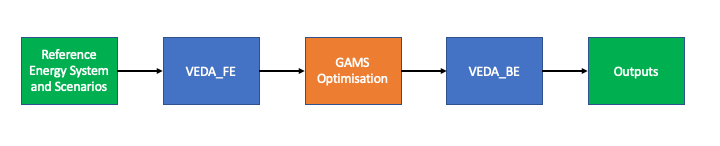
\includegraphics[width=\textwidth]{TIMES.png}
	\caption{TIMES Implementation Process}\
	\label{fig:times}
\end{figure}

The VErsatile data analyst (VEDA) \cite{VEDA} is a software package required for TIMES modelling. 
VEDA is an interface to design energy systems from Excel-based inputs and create the TIMES data and model text files for optimisation using GAMS.
The installation of VEDA FE and VEDA BE required a windows operating system. A virtual private network (VPN)
and Microsoft Remote Desktop was used to access a windows operating system via a virtual machine. GAMS Studio was installed on both 
the local Macintosh operating system and remote Windows operating system to perform the optimisation formulated in GAMS.
VEDA is proprietary and requires a commercial license to use. 
Fortunately, there is a 60 day trial version available for download and use.
After installing VEDA, GAMS and Microsoft Excel, I began following a TIMES user manual written by the IEA to build a standardised TIMES model.
The user manual started with a very basic energy system, incrementing on the energy model with twelve demo models.
I downloaded these twelve demo models to edit their associated Excel files.

The first stage was to adapt the existing Excel files so the user can design their own reference energy systems and sets of energy scenarios. 
Data and assumptions for reference energy systems and scenarios are primarily recorded in several tables across separate excel sheets and files.
I made copies of these excel files and began writing functions to change the data stored in these sheets and create user defined energy systems.

The second stage was to design energy systems using the VEDA interface. Figures

\begin{figure}[H]
    \centering
    \subfloat[Energy System Base Year]{{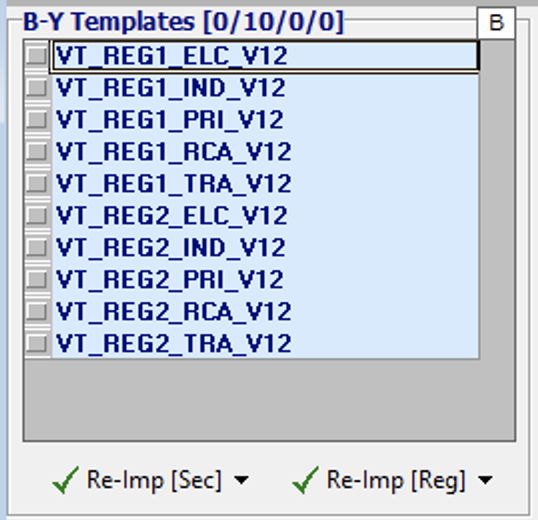
\includegraphics[width = 0.5\textwidth]{VEDABASE.png} }}
	\subfloat[Energy Scenarios]{{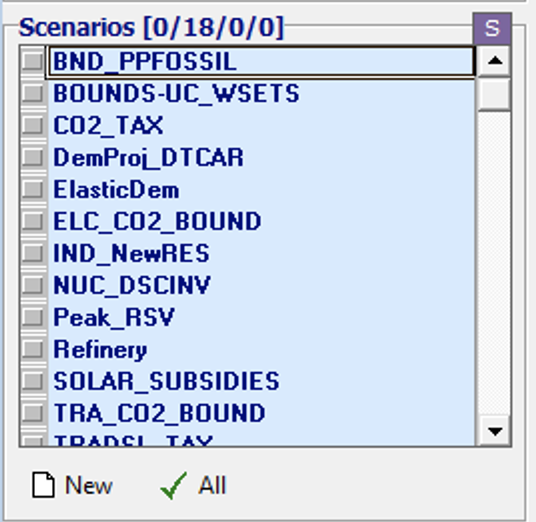
\includegraphics[width = 0.5\textwidth]{VEDAScenarios.png} }}
	\hfill
    \subfloat[Trade Relationships]{{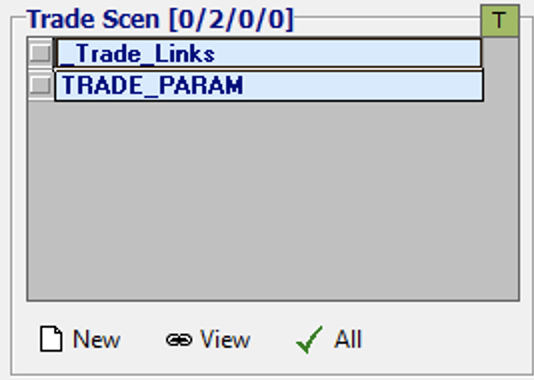
\includegraphics[width = 0.5\textwidth]{VEDATrade.png} }}%
	\subfloat[New Resources]{{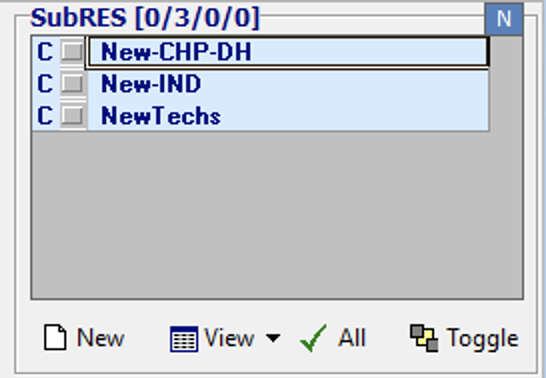
\includegraphics[width = 0.5\textwidth]{VEDAResources.png} }}%
	\hfill
	\subfloat[]{{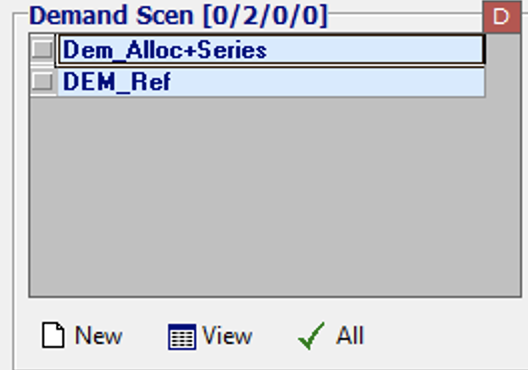
\includegraphics[width = 0.5\textwidth]{VEDADemand.png} }}
    \caption{VEDA Interface for building Energy Systems}%
    \label{fig:MFL}%
\end{figure}

The implementation of TIMES was difficult given several factors: 
The operating systems required to run the software. 
The integration of several software packages in both local and remote infrastructure.
The remote nature of online learning creating accessibility issues.



\subsubsection{OseMOYSIS}\label{OseMOSYS}
The combined use of both the OseMOSYS methodology and CPLEX solver required the formulation of an lp-format file by combining user-defined data and model text files.
These files are written in GNU Mathprog, a language intended for describing linear mathematical programming models \cite{GNU_Mathprog}. 
The OseMOSYS model file is stored in an excel sheet to make the OseMOSYS methodology transparent for the user. 
The model structure is converted into the required text file using the CreateModelFile function in the GOCPI package.
GNU Mathprog is a subset of the Algebraic Mathematical Programming Language (AMPL) \cite{AMPL} and consists of user-defined sets of statements and data blocks.
The custom anaconda environment (\textbf{osemosys}) was created to facilitate this model formulation. This environment contains the libcxx package which provides a standard library of C++ functionalities.
The GNU Linear Programming Kit (GLPK) sits within this library. GLPK uses GNU Mathprog to solve large-scale linear programming (LP), mixed integer programming (MIP), and other related problems. 
GLPK is called using the \textbf{glpsol} command in the osemosys conda environment:\
\begin{align*}	
	\textbf{glpsol -m model.txt -d data.txt --wlp GOCPI.lp}
\end{align*}
The correct installation of the GLPK was tested using the Utopian example data and model files using the aforementioned glpsol function.
The necessary lp-format file was generated for the CPLEX solver. 
This was paramount before disembarking on developing a standardised energy systems development method to generate both text and data files from a user-defined energy systems.
\subsection{Standardised Forecasting Methodology: GOCPI Package Development}
\subsubsection{Navigation Module}
\subsubsection{EnergySystems Module}
\subsubsection{CreateCases Module}
\subsubsection{Forecasting Module}
\subsubsection{Optimisation Module}
\subsection{Forecasting Energy Systems}
\subsubsection{Utopia Example}
\subsubsection{NZ Example}

\subsubsection{Energy System Functions}
Many functions were to enable scalable energy system modelling. 
The most important functions are highlighted in this section.
The function \textbf{def set\_discount\_rate} calculates the discount rate for each region.
This function is most important as the discount rate underpins the total value of discounted cash flows and the objective function.
The discount rate is calculated using the weighted average cost of capital (WACC) method.
The WACC, cost of equity, cost of preference equity and pre-tax cost of debt are calculated as follows:
\begin{align}
	WACC &= \frac{D}{E+D+K}\times r_d \times (1-t) + \frac{E}{D+E+K}\times r_e + \frac{K}{D+E+K}\times r_k
\end{align}
\begin{align}
	r_e &= r_f + \beta \times (r_m - r_f)\\
	r_d &= \frac{i}{D}\\
	r_k &= \frac{Div}{MV_{ps}}
\end{align}
\begin{equation*}
	\begin{split}
		&D= \text{Book value of debt (\$m)}\\
		&r_f= \text{Risk free rates (\%)}\\
		&K= \text{Market value of preferred equity (\$m)}\\
		&r_d= \text{Pre-tax cost of debt (\%)}\\
		&r_e= \text{Cost of ordinary equity (\%)}\\
		&Div= \text{Preference Dividends (\$)}\\
		& MV_{ps}= \text{Market value of preference shares (\$)}
	\end{split}
\quad\quad
	\begin{split}
		&r_k= \text{Cost of preferred equity (\%)}\\
		&t= \text{Effective tax rate (\%)}\\
		&i= \text{Cost of borrowings (\%)}\\
		&\beta= \text{Market risk co-efficient (\%)}\\
		&r_m= \text{Market return (\%)}\\
		&E= \text{Market value of equity (\$m)}
	\end{split}
\end{equation*}

The regions used in the energy system example are New Zealand and Australia. 
Both are public entities in this case.
The model may be used for both private and public entities.
It is assumed the financial performance and position for each region, reported in the the New Zealand and Australian Government's financial reports, are suitable for providing the financials necessary for calculating discount rates.
Cost of borrowings (i), Equity (E),  Debt (D) and Preference Equity (K) 
are reported in each region's annual financial reports (New Zealand \cite{TNZ_FR} and Australia \cite{AG_FR}).
It is assumed both have no preference shareholders, do not distribute preference dividends (Div), list preference shares ($MV_{ps}$) or have preference equity (K).
The effective tax rates (t) are each region's company tax rate. 
This example assumes New Zealand's market value of equity (E) is zero as not publically traded and Australia's negative net work implies market equity (E) is zero.
Risk free rates ($r_f$) were derived from average 10 Year Government bond yields using data from each region's respective 
Reserve Bank (Reserve Bank of New Zealand \cite{RBNZ_WIR} and Reserve Bank of Australia \cite{RBA_ZCL}). 
The monthly market returns for each region are annualised to calculate the market return ($r_m$). 
Each regions has a market index which serves as a proxy for the market. 
New Zealand has the NZX 50 and Australia has the ASX 200 \textbf{[Insert NZX50 and ASX200 references later]}.
Monthly returns are annualised as follows: 
\begin{align}
	\text{Annualised Monthly Return} = ((1 + \frac{\text{Index}_{\text{Ending}}-\text{Index}_{\text{Beginning}}}{\text{Index}_{\text{Beginning}}})^{(\frac{12}{\text{Number of Months}})})-1
\end{align}
The cost of ordinary equity is calculated using the Capital Assets Pricing Model (CAPM). 
Both New Zealand and Australia are assumed to have market risk co-efficients ($\beta$) of zero as their fiscal policy is market independent.
This methodology is appropriate for both public and private entities.
\subsection{User Interface Model Access}
\newpage
\section{Results}
\newpage
\section{Discussion}
\newpage
\section{Future Work}
\subsection{Python Development}
\subsection{NZ Example Completion}
\subsection{Develop Simulation Processes}
\subsection{Develop Investment Strategies}
\newpage
\section{Summary and Conclusion}
\newpage
\section{Reflection}
\newpage
\section{Appendices}
\subsection{Project Modules}
\subsection{OseMOSYS Model}
The Open Source Energy Modelling System is a linear programme with sets, parameters, an objective function and constraints related to energy systems.
The model is described below. Please refer to GOCPI OseMOSYS Structure.xlsx in the GitHub Repository for full descriptions of the sets, parameters and constraints.
%\lstinputlisting{"/Users/connor/Google Drive/Documents/University/Courses/2020/ENGSCI 700A&B/GOCPI/data/Inputs/GOCPI OseMOSYS/GOCPI_OseMOSYS_Model.txt"}
\newpage
\section{References}
\printbibliography
\end{document}